\chapter{Project Scheduling}
\begin{spacing}{1}
\setlength{\parskip}{0.3in}
\graphicspath{{./Chapter5/}}

\section{Introduction}
Project scheduling is structured listing of tasks, resources and duration  in a time sequenced manner so that the progress can be tracked and the project can be completed on time. Effective project schedule is a critical component of successful time management.
Schedule not only defines the start and end time of each activity or task, it also defines the dependencies among the tasks and the sequence of dependent tasks. A project schedule is created on the early planning phase of the project life cycle and is crucial in the project plan, where the schedule plan, schedule baseline, deliverable and requirements are identified. The project schedule is the guideline to the developer team throughout the execution phase. During the execution phase, the schedule baseline is compared against the actual progress and further modifications are added to the plan. Project scheduling is an iterative process.

\subsection{Scheduling Objectives}
A project schedule is a document that involves all the efforts needed to complete the project on time. It is also not possible to make an effective resource and cost management without a full and accurate work schedule. An effective project schedule provides a better resource and time management scheme and finds a trade off among its primary and secondary objectives.

\begin{itemize}
	\item \textbf{Primary Objectives}
	\begin{enumerate}
		\item \textbf{Best time} \newline Project schedule answers when an activity should start, how long it can take to complete and the deadline to finish the activity. 
		\item \textbf{Least cost} \newline Project schedule defines the what resources are associated with each activity and answers the lowest possible costs to complete each activity in the project.
		\item \textbf{Least risk} \newline Project schedule defines the slack and float available with each activity and dependencies among the activities to maintain.  
	\end{enumerate}
	\item \textbf{Secondary Objectives}
	\begin{enumerate}
		\item \textbf{Propose and evaluate different schedule alternatives} \newline Analyze different sequences of tasks and different schedule for their dependencies.
		\item \textbf{Make an effective use of resources} \newline Schedule the tasks in an cost effective manner so that no resources remain idle for a long period of time.
		\item \textbf{Reduce communication overhead among resources} \newline Project schedule organize the tasks in effective manner so that the resources are well distributed and available to all the components.
	\end{enumerate}
\end{itemize}

\section{Schedule Techniques}
Highly accurate estimation of duration of project tasks is the key concept to create a realistic project schedule. To make accurate estimations, project managers need to discuss with different stakeholders, review their perspectives on the tasks difficulty and possible duration, analyze previous projects and historic data. Alongside project managers follow different scheduling techniques to increase accuracy of their estimations of time and costs. 
Among different scheduling techniques, \textbf{Network Diagrams} uses to graphically represent the tasks of the project and their relationships. \textbf{CPM} and \textbf{PERT} are widely used network diagrams. The \textbf{CPM or Critical Path Method} is an equation that shows the possible longest timeline of the project. The \textbf{PERT or Program Evaluation and Review Technique} is used to visualize the flow of tasks for better estimations and also includes the dependencies.
 A \textbf{Work Breakdown Structure or WBS} is a graphical representation of decomposed tasks and deliverable of the final project. WBS becomes input to many other techniques, specially in the scheduling process. All the steps of the project are outlined in the organizational chart of a work breakdown structure.
 Another popular schedule technique is \textbf{Bar charts}. \textbf{Milestone Charts} is used to graphically represents the tasks in a temporal sequence, the bar length is directly proportional to the duration of that tasks. Another widely used technique is \textbf{Gantt Chart}. Gantt chart is also visualize the temporal sequence of tasks as milestone chart but gantt chart also shows the groups and subgroups of the tasks, dependencies among the tasks and can also shows the progress of each tasks. Gantt chart gives a more details view of the tasks sequence in temporal order.
 
 \subsection{Work Breakdown Structure}
 A work breakdown structure or WBS is visual, structured and hierarchical deconstruction of a project. WBS allows the team to work backward from the final deliverable of a project and identify all the activities needed to achieve a successful product. WBS takes a complex and large project and break down the project scope into more manageable pieces to make it easier to plan, schedule and deliver. WBS is the first step in the project scheduling process and provide the input for further estimation and scheduling techniques. A well structured WBS is created with several key components and some major components are as following:
 \begin{itemize}
 	\item \textbf{WBS Dictionary} \newline
 	A document that defines various elements of the WBS. It helps the team and stakeholders to understand the phases and deliverables.
 	\item \textbf{Task Number and Description} \newline Each task is assigned against a number to easily identify and refer the task in later processes. A description is the detail statement about the task.
 	\item \textbf{Task Dependency} \newline Some tasks have dependencies on other tasks as the dependent task have to wait until some other tasks have been completed. WBS defines the dependencies of each task(if any) in a well mannered way.
 	\item \textbf{Estimated Time Duration} \newline WBS tracks the estimated duration of each task, the start and end date of the tasks so that the tasks can be completed in time.
 	\item \textbf{Task Status} \newline WBS keeps record of the status of each task so the overall work progress can be measured. It is an iterative process and maintained throughout the execution phase.
 \end{itemize} 

As the proposed new system for the AKASH DTH is decomposed in a well structured WBS with each tasks number, description, duration and dependencies. This document works as the map for the project workflows and goals and further used in the CPM, PERT and Gantt Chart techniques. \newline
Time duration of each task is estimated using the top-down approach. The historic data gathered from their previous system's management was a key resource for the estimation and also expert judgment was asked from the previous team before planning the WBS. The dependencies were listed with additional care as the breakdown of the complex project scheduling highly affects from the internal dependencies among the component tasks. WBS was reviewed and the estimations were adjusted by Akash DTH team members.

\begin{table}[H]
\begin{center}
	\begin{tabular}{| p{1cm}|p{7cm}|p{2cm}|p{3cm} |}
		\hline
		Task ID & Task Description & Est. Duration & Dependencies \\
		\hline
		A & Analysis new proposed data models and functionalities & 14 days & -- \\
		\hline
		B & Designing UI & 21 days & A \\
		\hline
		C & Creating new database tables in a isolated environment & 21 days & A \\
		\hline
		D & Testing new database models integrity and relationships & 15 days & C \\
		\hline
		E & Coding new permission scheme & 15 days & C \\
		\hline
		F & Coding new customer service module & 15 days & C \\
		\hline
		G & Coding new custom package creation and alteration scheme & 15 days & C \\
		\hline
		H & Integrating UI with back-end API endpoints & 28 days & B,  J \\
		\hline
		I & Migrating new database models to production database system & 14 days & D \\
		\hline
		J & Testing back-end API endpoints & 21 days & I, E, F, G \\
		\hline
		K & Testing final UI & 14 days & H \\
		\hline
		L & Testing security features & 21 days & K \\
		\hline    
	\end{tabular}
\end{center}
\caption{WBS chart for proposed system of Akash DTH }
\label{chart:WBS}
\end{table}
  
\section{Network Diagrams}
Network diagrams is a graph like visual representation of the tasks in the WBS chart with the internal relationships and dependencies among the tasks. Network diagrams is a vital tool for the project scheduling and further measuring the work progress. Both the \textbf{CPM} and \textbf{PERT} techniques uses the network diagram technique for project scheduling. Two common methods to represent network diagram are \textbf{AON} or Activity On Node and \textbf{AOA} or Activity On Arrow. For scheduling the proposed system improvement for Akash DTH, we used both AON and AOA graph representations.

\paragraph{Activity On Arrow(AOA) Format}
On activities on arrow or AOA graph format, circles represent the events like start and end of a connected task, and lines represent the tasks. Time goes the direction of the arrow, generally from left to right. Duration and description of a task can be added in the label of the respective line. AOA method is also generally known as \textbf{Arrow Diagramming Method(ADM)}. AOA network graph for the  WBS listed in the table \ref{chart:WBS} is shown in Figure \ref{fig:aoa}.

\begin{figure}[H]
	\centering
	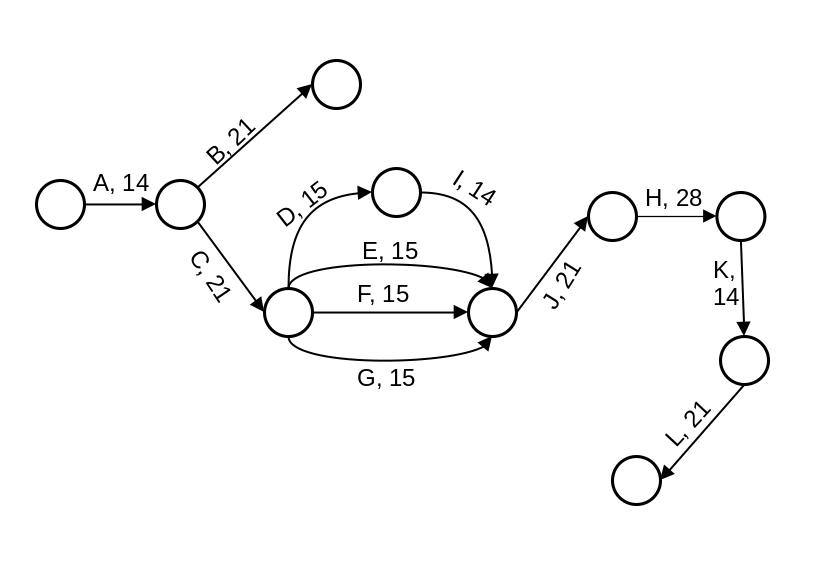
\includegraphics[width=0.8\textwidth]{AOA}
	\caption{AOA network graph}
	\label{fig:aoa}
\end{figure} 

\paragraph{Activities On Node(AON) Format}
On activities on node or AON network, nodes are either presented with a circle or rectangle, task duration, description, start, end dates are presented also in the nodes and arrows represent the dependencies among the connected nodes ar tasks. AON is also popularly referred as \textbf{Precedence Diagramming Method (PDM)}.A simple AON network graph for the WBS in the table \ref{chart:WBS} is shown in Figure \ref{fig:aon}.

\begin{figure}[H]
	\centering
	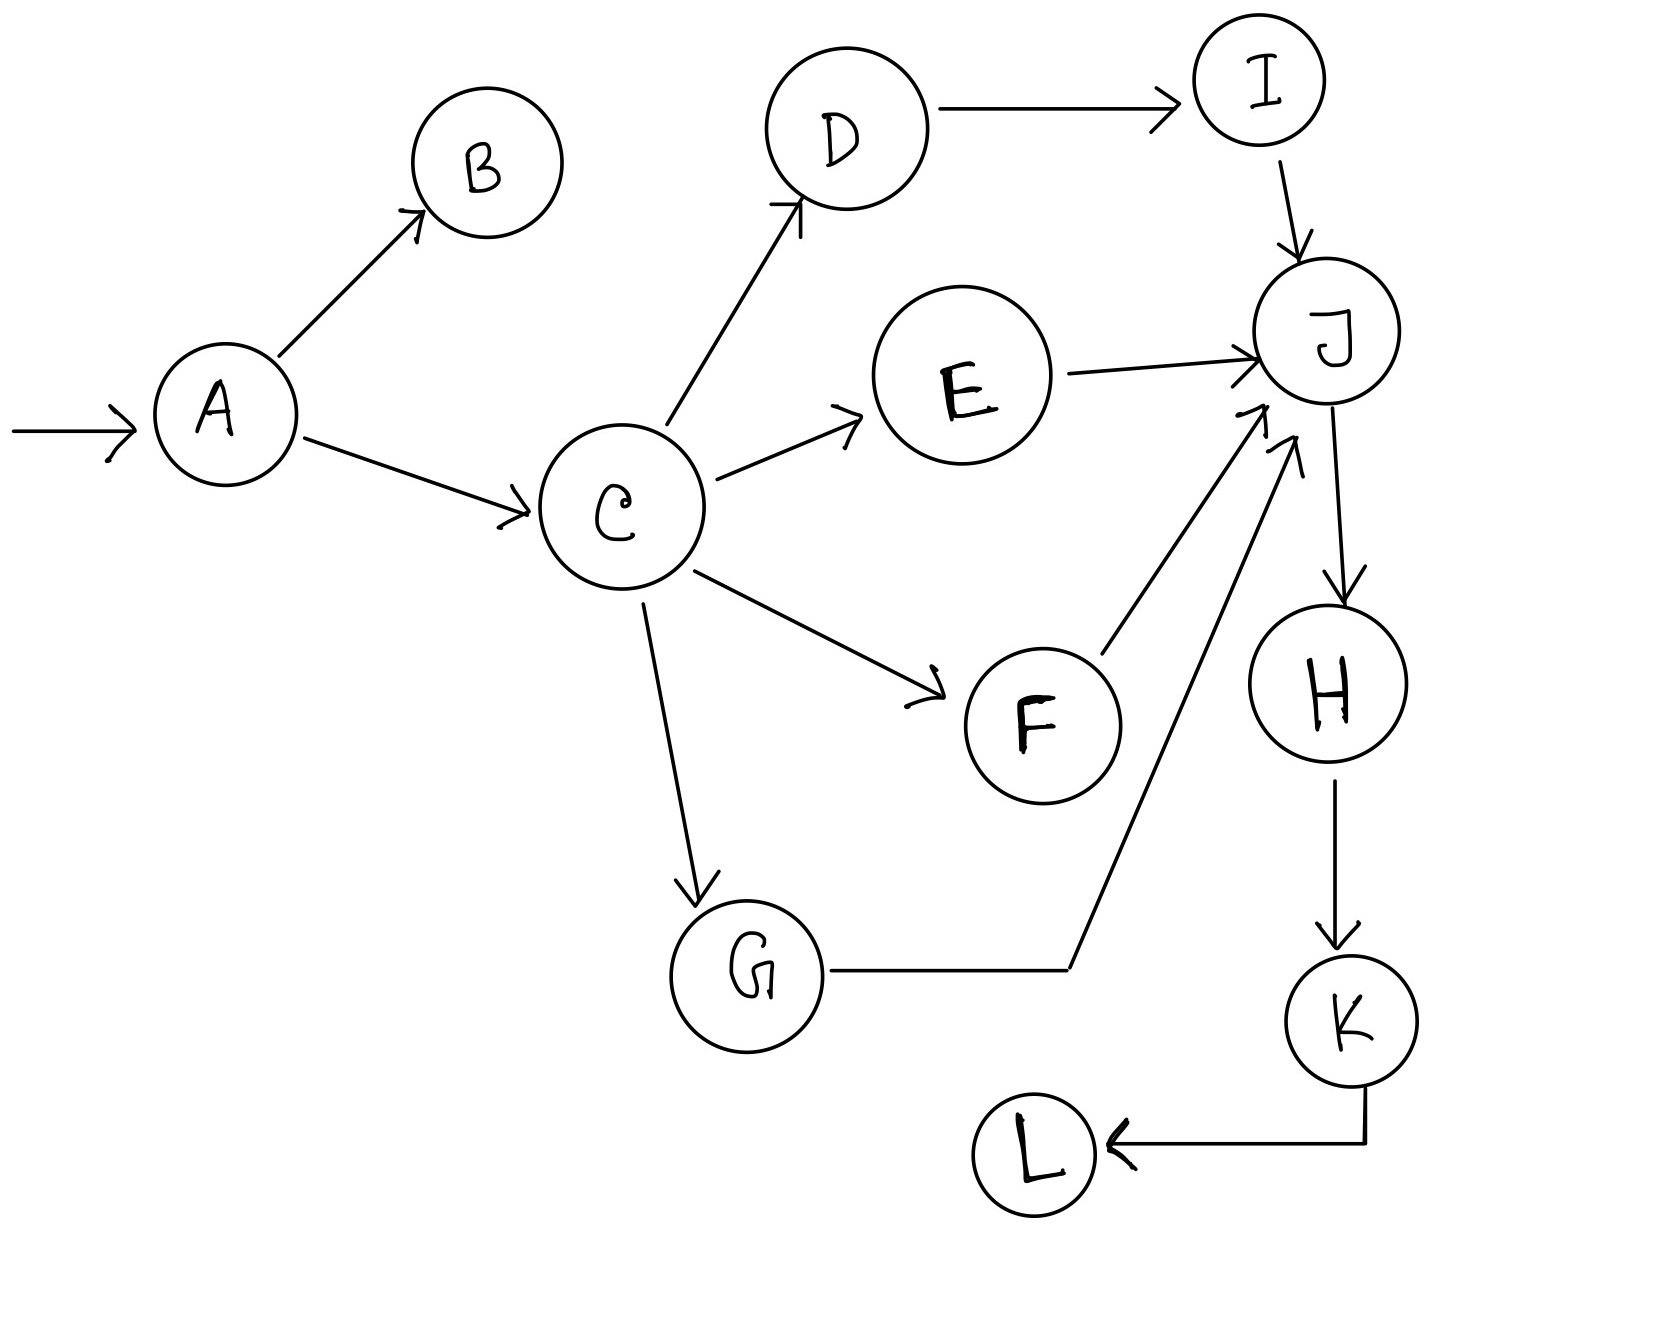
\includegraphics[width=\textwidth, height=3in]{AON}
	\caption{AON network graph}
	\label{fig:aon}
\end{figure} 

\subsection{Critical Path Method(CPM)}
\subsubsection{Critical Path}
Critical path in a project is sequence of the tasks that directly effects in the project completion deadlines. That means any delay in a task of the critical path will eventually create a delay in the final project completion. So critical path detects the minimum time needed to complete the project. Each project must have at least one critical path but more than one critical path is also common in project management. Accelerate the tasks on the critical path does not guarantee to shorten the project duration as the critical path can be shifted to a new path. Tasks that are not part of the critical path have a little impact on the project completion time. Some key concepts associated with critical path are listed below:
 
 \paragraph{Early Start Time(ES)} 
 This is earliest possible time a start can be started. A task early start time will always after the preceding task's early finish time. When a task have multiple preceding tasks, the maximum of their early finish time is used as the task's early start time.
 \paragraph{Early Finish Time(ET)}
 This is earliest possible time a task can be finished. Early finish time is simply the early start time plus the estimated duration of the task.
 \paragraph{Late Start Time(LT)}
 This is last minute a task can be started without affecting the project schedule. Late start time is simply the late finish time minus the duration of the task.
 \paragraph{Late Finish Time(LF)}
 This is the last minute a task can be completed within the project schedule. A task's late finish is the late start time of succeeding task's late start time, if the task has multiple successor then minimum of their late start is used as the late finish of the current task.  
 \paragraph{Slack}
 This defines how long a task can be delayed without affecting the project schedule and finish deadline. All tasks in the critical path will have a zero slack and other tasks that are not in the critical path will have a positive slack.
 
 All these information are vital in critical path determination and project scheduling. So in the network diagram we used a rectangular node representation including the tasks number, duration, early start, early finish, late start, late finish and slack of the task as the following structure.
 
 \begin{center}
\begin{tabular}{|c|c|c|}
	\hline
	ES & Duration & EF \\
	\hline
	\multicolumn{3}{|c|}{Project ID} \\
	\hline
	LS & Slack & LF \\
	\hline
\end{tabular}
\end{center}


\subsubsection{Creating CPM Network Diagram}
Critical path method is the algorithm to detect the critical path in the project schedule. It uses the slack of the tasks to detect the critical path. CPM is a two phase algorithm, a forward pass and followed by a backward pass.

\subsubsection{Forward Pass} 
In the forward pass, we calculate the early start(ES) and early finish(EF) of each task. In forward pass, we started the calculation from the left most task or the starting task(the task has no dependency) and proceed to the right until the final task reached. The first step in the forward pass is to create the network diagram using the WBS listed in table \ref{chart:WBS}. ES of an activity is equal to the EF of it's predecessor or the maximum of the EF(s) if it has multiple predecessors. ES of the first or leftmost task is always zero. The formula used to calculate EF is, $EF = ES + duration.$

\subsubsection{Backward Pass}
In backward pass, we calculate the late start(LS) and late finish(LF)  of each task. We started from the last or final task of the schedule and moved to preceding task, in a backward direction. The LF is determined first, then LS is calculated from LF and duration. The LF of a task is equal to the LS of the succeeding task or the minimum of the LS if multiple succeeding  tasks are there in the project schedule. The LF of the final task is equal to the EF of that task previously determined in the forward pass phase. The formula used to calculate LS is, $LS = LF - duration.$

\subsubsection{Slack and Critical Path Identification}
After the backward pass, all the information ES, EF, LS, LF of each task has been determined. The next step is the slack calculation. Slack identifies the tasks belong to the critical path. The formula used tor slack calculation is,$ slack =  LS - ES = LF - EF $. When slack is calculated, critical path is identified with tasks slack equals to zero. 

The CPM network diagram for our project schedule is shown in Figure \ref{fig:cpm}. 

\begin{figure}[H]
	\centering
	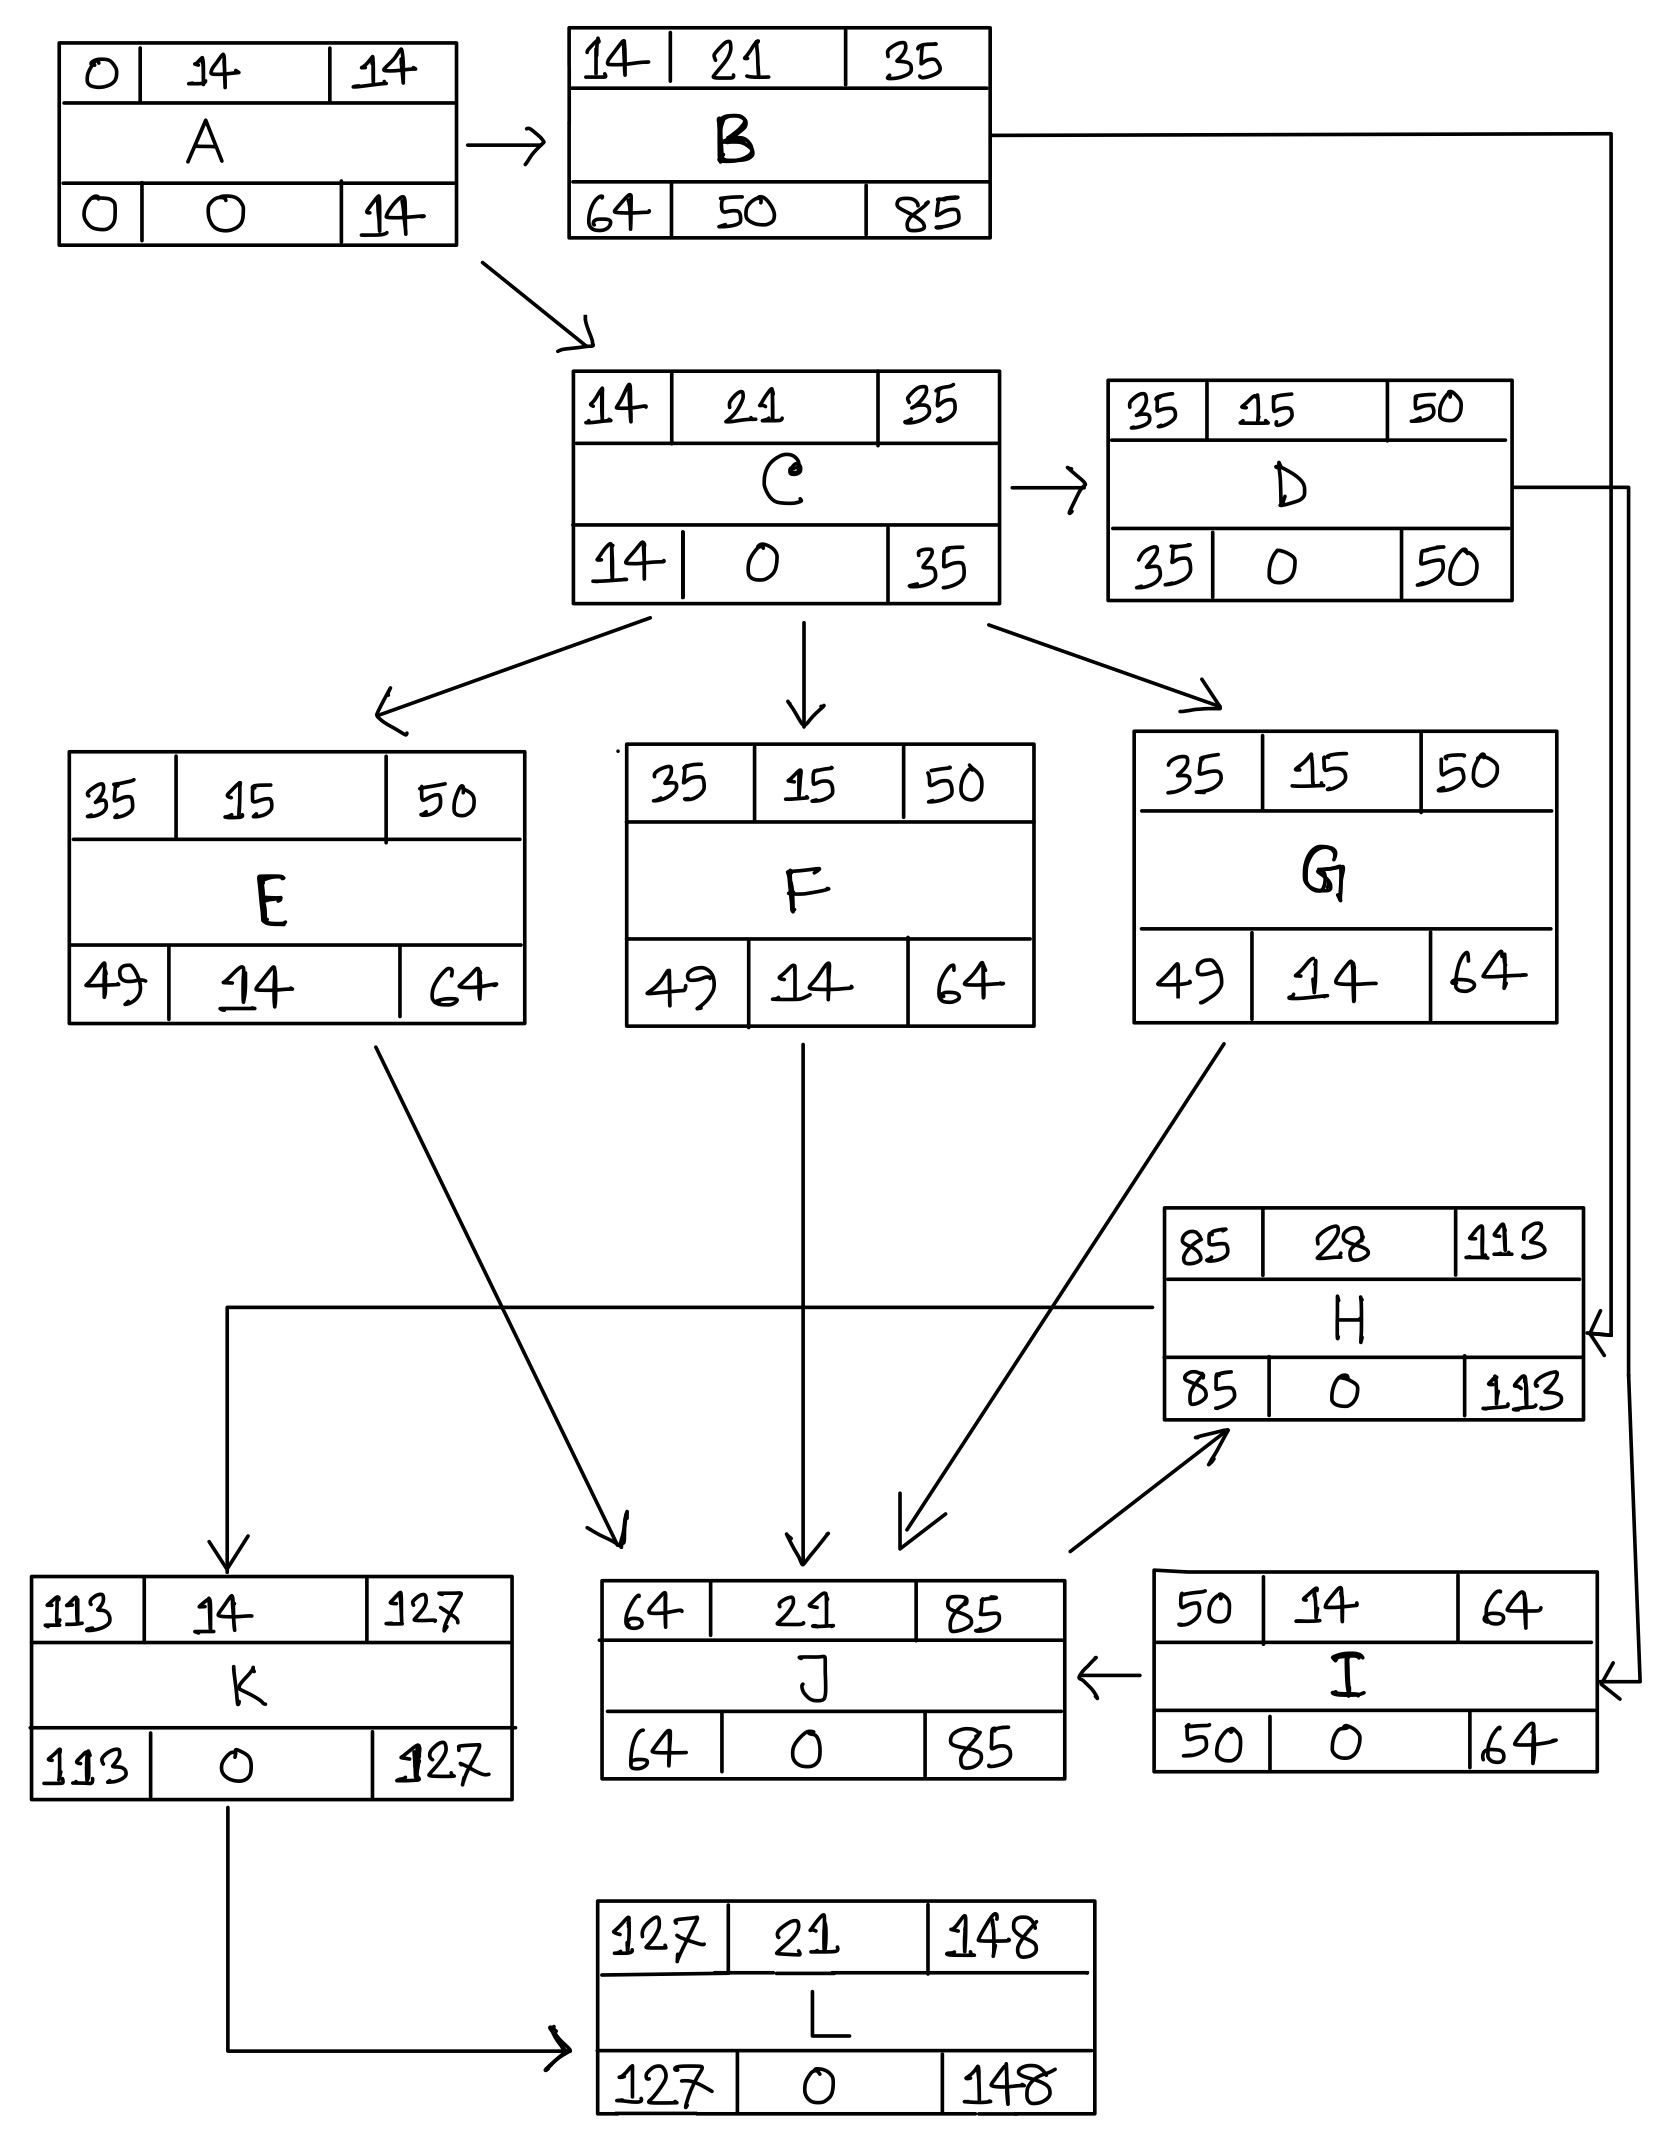
\includegraphics[width=0.8\textwidth]{CPM}
	\caption{CPM network diagram}
	\label{fig:cpm}
\end{figure}

From the above network diagram, we can identify the critical path in our project schedule where the tasks in path have a slack equals to zero. Critical path of schedule for Akash DTH's improvement project : \newline
\[ A \to C \to D \to I \to J \to H \to K \to L \]

\subsubsection{Summary Of CPM}  
CPM is a great tool for project scheduling. With CPM diagram, we can reveal and show the dependencies among the tasks in our schedule. Every task is associated with the slack time, so we can determine which tasks can be delayed and we are able to make changes on our project management, like reallocating team members and resources. With CPM technique our project schedule become more realistic.
Some disadvantages to use CPM in our project schedule were, the complexity of CPM. Our proposed system project is more complex as their are several dependencies on some tasks and as a result the network diagram grows larger. Maintaining a large network diagram is more difficult. CPM lacks the way to keep track of the progress of the tasks in execution period. 

\subsection{PERT}
Program evaluation and review technique or PERT is a network diagram to represent the project's timeline. PERT method uses three estimations to calculate the expected time of each task. PERT is more effective when the duration of activities are uncertain. A brief description of each of three estimations used in PERT is given below:
\begin{itemize}
	\item \textbf{Optimistic Time, $a$} The minimum amount of time at least required to complete a task. This represent the best case scenario time.
	\item \textbf{Pessimistic Time, $b$} The maximum of time time a task can be taken to complete. The represent the worst case scenario time.
	\item \textbf{Most Likely Time, $m$} The best estimate of how long a task can take to complete assuming there is no delay or scarcity of resources.
\end{itemize} 

After finalize these three estimations, the expected time $te_{i}$ is calculated using the following formula of weighted average: \newline
\begin{equation}
te_{i} = \frac{a_i + 4m_i + b_i}{6} 
\end{equation}

Then the standard deviation $SD_{i}$ of each task is calculated. Standard deviation or SD signifies the variance of expected time of the tasks, smaller standard deviation means the value to be more close to the mean and the estimation is more confident. The formula used to calculate standard deviation is \newline

\begin{equation}
SD_{i} = \frac{b_{i} - a_{i}}{6} 
\end{equation}

In PERT method, expected time and standard deviation for each task is calculated individually and then the critical path is identified and finally the expected time and standard deviation for the whole project is calculated using every task present in the critical path.
Expected time of the project, assuming their are n number of tasks in the critical path of the schedule: \newline

\begin{equation} \label{eq:3}
 te_{cd} = \sum_{i=1}^{n}te_i
\end{equation}

 And the standard deviation of the project will be  \newline

\begin{equation}
SD_{cp} = \sqrt{\sum_{i=1}^{n} SD_i^2} 
\end{equation}

\subsubsection{PERT Activity List}
PERT activity list is tabular method that shows the activities their three estimations, expected time and standard deviation in a table format. We used the activities or tasks previously decomposed in WBS(Table \ref{chart:WBS}) and make the optimistic, pessimistic and most likely estimations of each task and then calculated their expected time and standard deviation. Estimations were make using top-down method and using historic data and expert evaluation. The PERT list is presented in the table \ref{chart:PERT}. 

From the PERT activities list, tasks have standard deviation within the range 0 to +1.5 which signifies that the expected time is well estimated. Majority of the tasks standard deviation are in range 0 to +1.0, only one task has standard deviation over 1.0, which evens provide proof of the lower variance of our estimations. 

\begin{table}[h!]
	\begin{center}
		\begin{tabular}{| p{1cm} | p{2cm}| p{2cm} | p{2cm} | p{2cm} |p{2cm} | p{3cm} |}
			\hline
			Task ID  & Optimistic Time, $a_i$ &   Most Likely Time, $m_i$ & Pessimistic Time, $b_i$ & Expected Time, $te_i$ & Standard Deviation, $SD_i$ & Dependencies \\
			\hline
			A  & 12 & 14 & 16 & 14 & 0.67 & None \\
			\hline
			B  & 19 & 21 & 23 & 21  & 0.67 & A \\
			\hline
			C  & 18 & 21 & 24 & 21 & 1.0 & A \\
			\hline
			D  & 12 & 15  & 17 & 15 & 0.83 & C \\
			\hline
			E & 12 & 15 & 18 & 15 & 1.0 & C \\
			\hline
			F  & 13 & 15 & 18 & 15 & 0.83 & C \\
			\hline
			G  & 14 & 15 & 20 & 16 & 1.0  & C \\
			\hline
			H &  24 & 28 & 31 & 28 & 1.17 & B,  J \\
			\hline
			I  & 13 & 14 & 15 & 14 & 0.33 &  D \\
			\hline
			J  & 18 & 21 & 27 & 22 & 1.5  & I, E, F, G \\
			\hline
			K  & 12  & 14 & 15 & 14 & 0.5  & H \\
			\hline
			L  & 18 & 21 & 23 & 21 & 0.83 & K \\
			\hline    
		\end{tabular}
	\end{center}
	\caption{PERT activity list for proposed system of Akash DTH }
	\label{chart:PERT}
\end{table}

\subsubsection{PERT Chart}
PERT chart network diagram with AOA or Activities On Arrow representation. In PERT chart the nodes represent the project milestones and arrow represents the activity to be completed to reach the guided milestones.  Activity expected duration is also represented in the arrow. PERT uses the critical path we previously identified with CPM method $ A \to C \to D \to I \to J \to H \to K \to L $ in the network diagram. PERT chart for ours proposed system for AKASH DTH with the critical path highlighted is shown in figure \ref{fig:pert}.

\begin{figure}[H]
	\centering
	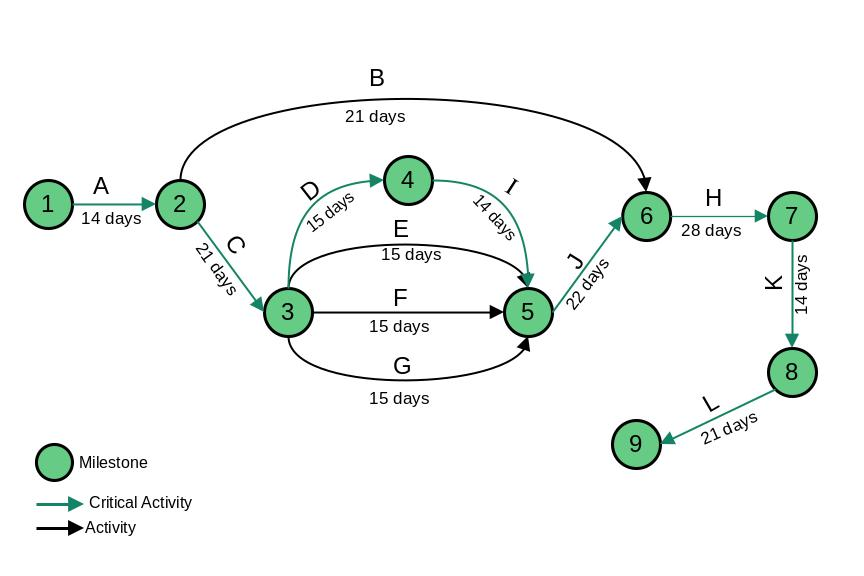
\includegraphics[width=0.8\textwidth]{PERT}
	\caption{PERT Chart for Akash DTH's project schedule}
	\label{fig:pert}
\end{figure} 
 
\subsubsection{PERT Analysis For Overall Project}
The expected duration of the overall project is the sum of the expected time of each task on schedule critical path. So expected time to complete our proposed work for Akash DTH is \newline

\begin{equation*}
	\begin{split}
		te_{cp} &= te_A + te_C + te_D + te_I + te_J + te_H + te_K + te_L \\
		&= 14 + 21 + 15 + 14 + 22 + 28 + 14 + 21 \\
		& = 149  days
	\end{split}
\end{equation*}

Standard deviation of the overall project basically signifies the variance of the whole project schedule estimations. To calculate the standard deviation of our proposed system for Akash DTH, we used the critical path identified previously in CPM method. 
So standard deviation of our project schedule,
\begin{equation*} 
	\begin{split}
		SD_{cp} &= \sqrt{SD_A^2 + SD_C^2 + SD_D^2 + SD_I^2 + SD_J^2  + SD_H^2 + SD_K^2 + SD_L^2 } \\
		&= \sqrt{0.67^2 + 1.0^2 + 0.83^2 + 0.33^2 + 1.5^2 + 1.17^2 + 0.5^2 + 0.83^2 } \\
		& = \sqrt{7.4934} \\
		& = 2.7374
	\end{split}
\end{equation*} 

So the overall variance in our project schedule increases because of some high deviation was introduced in some tasks in the critical path. So the estimations of the tasks included in the critical path affects the overall project estimation.

\subsubsection{Summary of PERT}
PERT is another great technique to schedule a project timeline. Main advantage of PERT for our project schedule was the uncertainty of our time estimation. As we are not well experienced in project management, our estimations are not enough realistic. PERT uses three estimations for a task and then expected time of a task is determined based on those estimations. Thus the variance of our estimations was able to be reduced and the result becomes more realistic. 
Main disadvantage of PERT in our project schedule was the labor it takes to make the estimations. Bad estimations increase the risk of higher variance in the resultant outcome. Making three estimations for each tasks of the project is thus an time and labor extensive process. It also requires recursive review and updates throughout the project management process.

\section{Bar Chart}
Bar charts are graphical viewing technique of task scheduled over time. Bar charts enable the team member to view start and end time, progress of the task in the comparison with current date. Gantt chart is the most used bar chart technique in project scheduling. We represent our proposed system development project schedule using a gantt chart. 
\subsection{Gantt Chart}
 Gantt chart is a bar chart which shows the tasks in temporal sequence with each task's duration and progress on the chart. Gantt chart also allows to represent the temporal dependencies among tasks even the task's allowed slack time. Some important analogy in gantt chart representation is briefly described below.
 \textbf{Precedence}\newline
 One task must be done before another task. Task A have precedence over task B or task A is predecessor of task B in figure \ref{fig:pecedence}
 \begin{figure}[h]
 	\centering
 	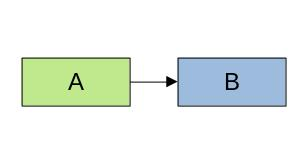
\includegraphics[width=0.4\textwidth]{Precedence}
 	\caption{Precedence in gantt chart}
 	\label{fig:pecedence}
 \end{figure} 

\textbf{Concurrent}\newline
Concurrent tasks are those tasks in the schedule that can occur concurrently. Concurrent tasks can be completely or partially overlapped. Both complete and partial concurrency of tasks shown in figure \ref{fig:conc}. 
\begin{figure*}[h]
	\centering
	\begin{subfigure}{0.4\textwidth}
		\centering
		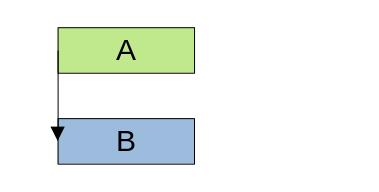
\includegraphics[height=1.5in]{c_ol}
		\caption{Complete Overlapped}
	\end{subfigure}
	\begin{subfigure}{0.4\textwidth}
		\centering
		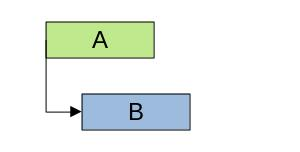
\includegraphics[height=1.5in]{p_ol}
		\caption{Partially Overlapped}
	\end{subfigure}
	\caption{Concurrent tasks in gantt chart}
	\label{fig:conc}
\end{figure*}
     
\subsubsection{Dependencies in Gantt Chart}
\textbf{Finish-to-Start, FS} A f-to-s B or A FS B means Task B can't start before task A finishes. Finish to start dependency in gantt chart is shown in figure \ref{fig:FS}.
 \begin{figure}[H]
	\centering
	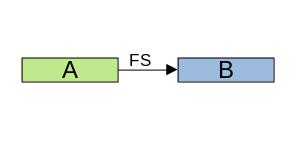
\includegraphics[width=0.4\textwidth]{FS}
	\caption{Finish-to-Start dependency}
	\label{fig:FS}
\end{figure} 
\textbf{Start-to-Start, SS} A s-to-s B or A SS B means Task B can't start until task A starts. Start to start dependency in gantt chart is shown in figure \ref{fig:SS}.
\begin{figure}[H]
	\centering
	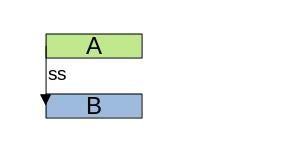
\includegraphics[width=0.4\textwidth]{SS}
	\caption{Start-to-Start dependency}
	\label{fig:SS}
\end{figure} 
\textbf{Finish-to-Finish, FF} A f-to-f B or A FF B means Task B can't finish before task A finishes. Finish to finish dependency in gantt chart is shown in figure \ref{fig:FF}.
\begin{figure}[H]
	\centering
	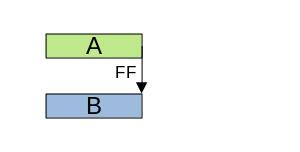
\includegraphics[width=0.4\textwidth]{FF}
	\caption{Finish-to-Finish dependency}
	\label{fig:FF}
\end{figure} 
\textbf{Start-to-Finish, SF} A s-to-f B or A SF B means Task B can't finish before task A starts. Start to finish dependency in gantt chart is shown in figure \ref{fig:SF}.
\begin{figure}[H]
	\centering
	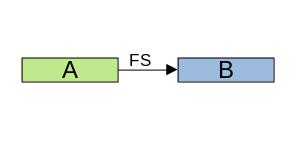
\includegraphics[width=0.4\textwidth]{FS}
	\caption{Finish-to-Start dependency}
	\label{fig:SF}
\end{figure} 

\textbf{Lag Time}\newline
Lag time means delay between sequenced tasks in the planned schedule. In gantt chart it is possible to shows lag time between tasks. Lag time in gantt chart is represented in figure \ref{fig:lag}.
\begin{figure}[H]
	\centering
	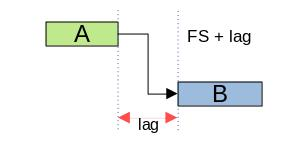
\includegraphics[width=0.4\textwidth]{lag}
	\caption{Lag time in gantt chart}
	\label{fig:lag}
\end{figure} 

\textbf{Lead Time}\newline
Lead time means advance between sequenced tasks in the planned schedule. In gantt chart it is also easy to shows lead time between tasks when a task starts before its schedule time. Lead time in gantt chart is represented in figure \ref{fig:lead}.
\begin{figure}[H]
	\centering
	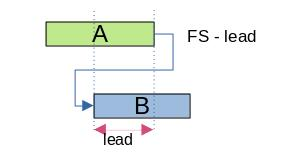
\includegraphics[width=0.4\textwidth]{lead}
	\caption{Lead time in gantt chart}
	\label{fig:lead}
\end{figure} 

\subsubsection{Slack}
Slack is a important measurement in project schedule. Slack of a task means the amount of time that task can be delayed with out causing any delay in the project compilation time. It is common for a task to have some slack when there are multiple concurrent task in project schedule. 
Free slack of a task is the amount of time the task can be delayed with out causing any further delay in any subsequent task. In figure \ref{fig:fslack}, free slack of Task B is where both task A and B have start-t0-finish dependency with task C and task A takes lnger time than task B that causing a free slack time for task B.
\begin{figure}[H]
	\centering
	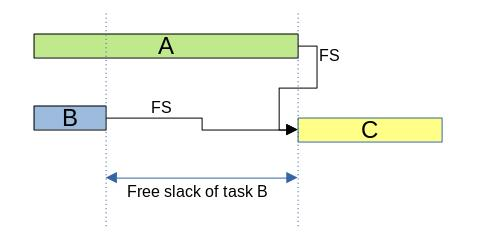
\includegraphics[width=0.6\textwidth]{fslack}
	\caption{Free slack in gantt chart}
	\label{fig:fslack}
\end{figure} 

Thus a gantt chart works as a great visual representation of project schedule for both team members and even non technical stake holders. We create a gantt chart for the project of Akash DTH system improvement using online based project management software, Instagantt. The gantt chart is shown in figure \ref{fig:gantt}.

\begin{figure}[H]
	\centering
	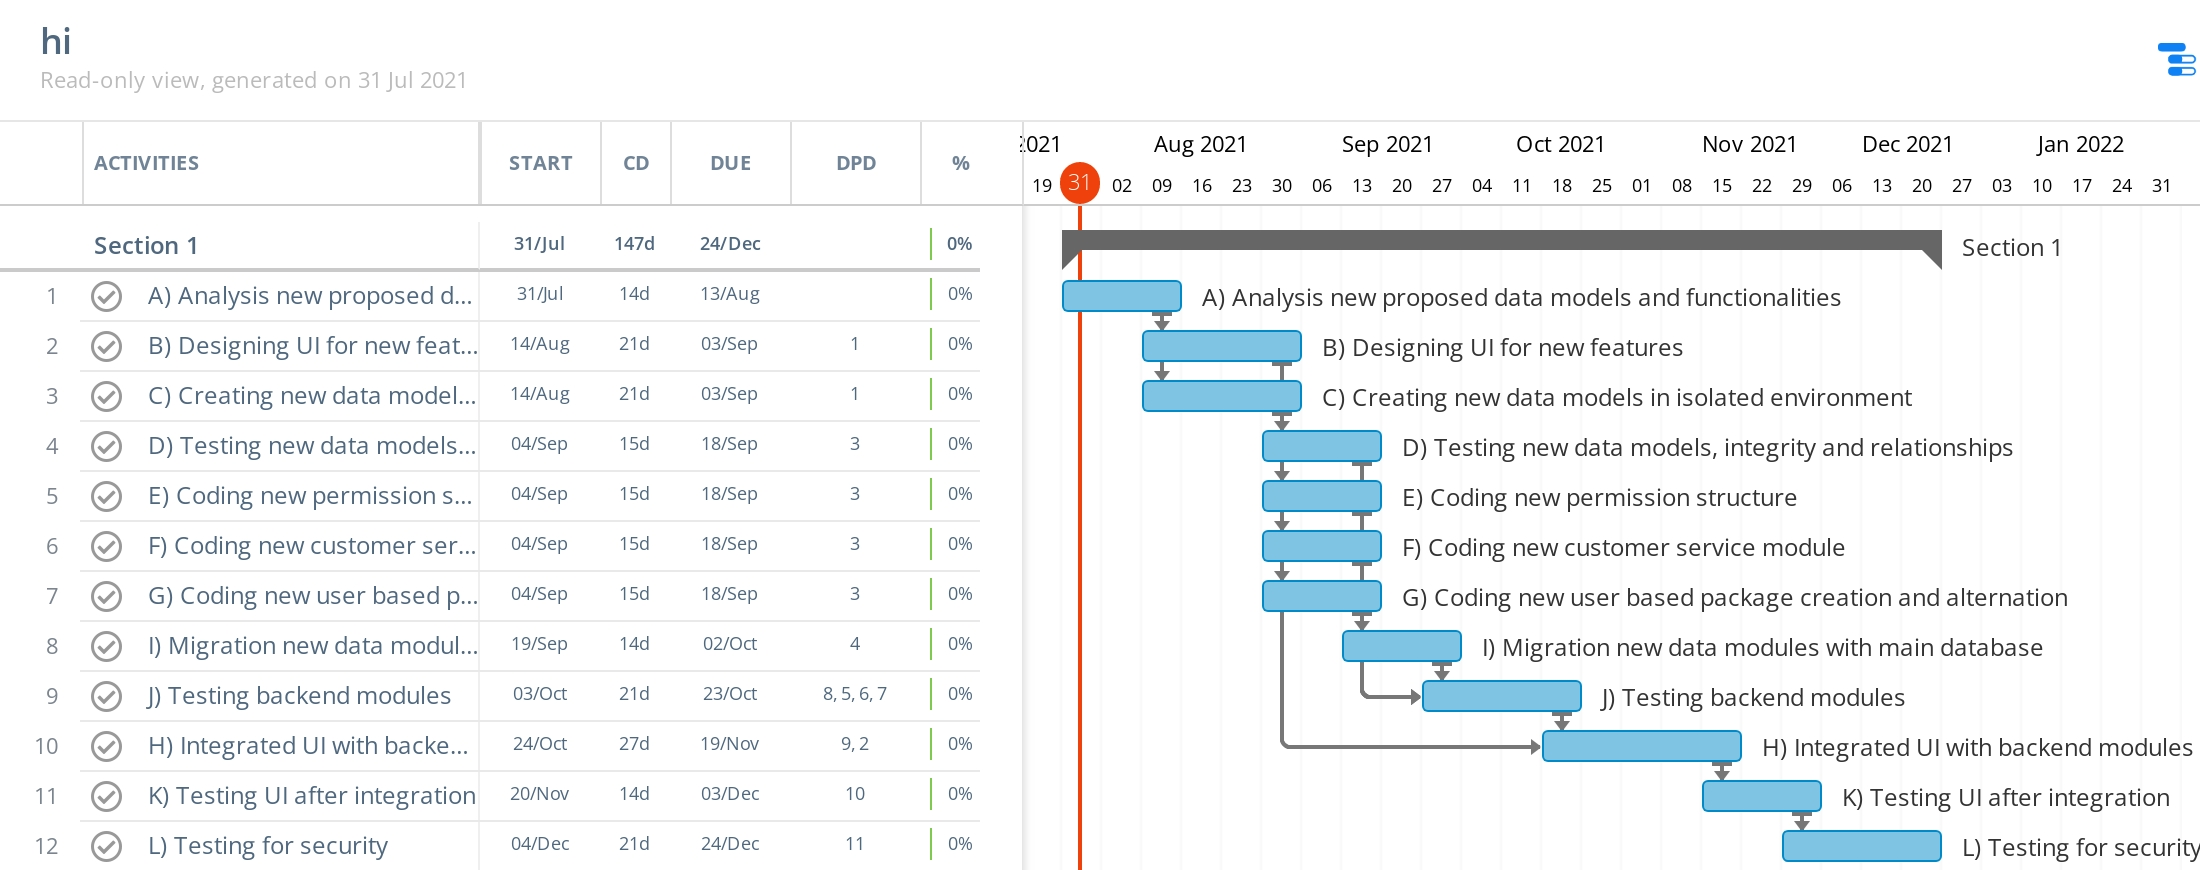
\includegraphics[width=\textwidth]{gantt}
	\caption{Gantt chart for project schedule}
	\label{fig:gantt}
\end{figure} 

\paragraph{Summary of Gantt Chart}
Gantt chartt help the team not only in the early project schedule and planning, is maintained through out the project duration to keep progress of the tasks and maintain deadlines. We developed a gantt chart for our proposed improvement project for Akash DTH, we assumed the project start date from 31 July, 2021 to develop the gantt chart. Gantt chart keeps notations of task progress and resources allocated to the task but lacks to represent the uncertainty associated with task duration estimations.  

\section{Schedule Optimization}
Project schedule is created in the planning phase of the project management and highly based on estimations. So several techniques are used in project schedule to optimize the planned schedule and shorten the project timeline. Among different optimization techniques some common techniques are,
\begin{itemize}
	\item Re-organize Schedule
	\item Reduce Project Scope
	\item Increase Cost
\end{itemize}
In our project for Akash DTH both re-organize and reduce scope techniques are not feasible. So we considered and proposed the increase cost technique to optimize our planned schedule if it becomes necessary to shorten the project completion time. 

\subsection{Increase Cost}
Cost increase a schedule optimization technique in which uses a trade off between cost and time. In case of we need to shorten our project duration cost technique can provide a better solution than any other optimization techniques. In cost increase we don't allow to reduce our project scope, reducing scope will also cause removal of the features we proposed to improve Akash DTH service. There ae two common ways to optimize schedule by creasing cost,
\paragraph{Crashing} We can allocate more resources to tasks. Like the team size can be increased in longer duration tasks to complete the task faster. Some tasks in our schedule critical path have a large expected duration, so this tasks will be possible to complete in a shorter time is more people engaged in the task and work in a team. Increase member in the development team will increase the cost of the project but completion time can reduced by a large factor by appointing experienced and confident team members.
\paragraph{Breaking Dependencies} Second method in cost increase schedule optimization is breaking the task dependency and allowing more concurrent tasks in the schedule. In our proposed schedule many tasks have multiple dependencies that make schedule more sequential and lengthen the project duration. By breaking the dependencies in those tasks will result in more concurrent tasks, though breaking dependencies will increase the risk of the project management and some dependencies must have to be maintained for a task to be completed successfully. Breaking dependencies will allow more concurrent tasks, and more concurrent  tasks will need more resources but shorten the overall duration. This this technique also trade off between cost and time to optimize the project schedule.

\section{Conclusion}  
Project schedule is a vital tool in project's time and resource management. Scheduling process starts in the early phase of project management and is maintained in the full duration of project completion. We planned the schedule by first creating the work breakdown structure chart, identifying the tasks and then estimating task duration. We created both CPM and PERT network diagram for this project schedule. Through CPM we can identified the critical path of the project. PERT was great tool for this project schedule because of the uncertainty we have in our estimated time duration. And then the Gantt chart of the schedule was developed which shows the duration and keeps the progress in real time. We accounted the risk of possible delay in the schedule as plans are not always perfect and considered cost increase method to optimize our planned schedule. Project schedule is not a one time job, it is an iterative process, so the planned schedule needs regular revision and further improvements in throughout the execution phase of project management.
  
\end{spacing}